%% Tudor Berariu, Alexandru Sorici
%% Noiembrie 2012


\begin{frame}
  \frametitle{Problema interpretării}
  \begin{block}{Problema interpretării unei secvențe de observații}
    Date fiind un model   \alert{$\lambda=(A,B,\Pi)$} și o
    secvență de observații \alert{$O = [ o_1 o_2 \cdots o_T ]$}, 
    cum alegem o secvență corespunzătoare de stări
    \alert{$Q_{\text{best}} = [ q_{1_{\text{best}}} q_{2_{\text{best}}} \cdots q_{T_{\text{best}}} ]$} care \emph{să
      dea un înțeles} observațiilor? Cum \emph{descoperim} partea
    ascunsă a modelului?
  \end{block}\pause
  \begin{itemize}
  \item Răspunsul depinde de criteriul cu care alegem \emph{cea mai bună} secvență\pause
    \begin{itemize}
    \item \alert{secvența celor mai probabile stări $q_{t_{\text{best}}}$} (luate individual), date fiind modelul și secvența observată:\\
      $q_{t_{\text{best}}} = \underset{s_i}{\operatorname{argmax}}\; P(q_t = s_i \vert O, \lambda)$
    \item \alert{cea mai probabilă secvență de stări $Q$} (per ansamblu), date fiind modelul și secvența observată:\\
      $Q_{\text{best}} = \underset{\text{all }Q}{\operatorname{argmax}}\; P(Q \vert O, \lambda)$
    \end{itemize}
  \end{itemize}
\end{frame}


\begin{frame}
  \frametitle{Secvența celor mai probabile stări}
  Notație: $P(q_t = s_i \vert O, \lambda) = \mathbf{\gamma_{t,i}} = 
  \frac{\alpha_{t,i}\beta_{t,i}}{\displaystyle\sum_{j=1}^{N}\alpha_{t,j}\beta_{t,j}}$
  \begin{itemize}
  \item Este un criteriu satisfăcător?\pause
  \item \textbf{NU!}\\Pot exista $q_t$ și $q_{t+1}$ astfel încât $a_{q_t,q_{t+1}}=0$
  \end{itemize}
    % \begin{itemize}      
  % \item How can we answer the \emph{best explanation} problem?  \pause
  % \item \textbf{Individually} most likely states
  %   \begin{equation}
  %     \label{eq:individually}
  %     \gamma_{t,i}=P(q_t = s_i \vert O, \lambda)
  %   \end{equation}
  %   \pause
  % \item Computation
  %   \begin{equation}
  %     \label{eq:gamma_formula}
  %     \gamma_{t,i}=\frac{\alpha_{t,i}\beta_{t,i}}{P(O\vert \lambda)} =
  %     \frac{\alpha_{t,i}\beta_{t,i}}{\displaystyle\sum_{k=1}^{N}\alpha_{t,k}\beta_{t,k}}
  %   \end{equation}
  %   \pause
  % \item Problems?
  % \end{itemize}

\end{frame}

\begin{frame}
  \frametitle{Algoritmul Viterbi}
  \begin{itemize}
  \item Criteriu care ia în considerare distribuțiile de probabilitate 
    ale tranzițiilor între stări
  \item Cea mai bună cale:
    $Q_{\text{best}} = [q_{1_{\text{best}}} q_{2_{\text{best}}} \cdots q_{T_{\text{best}}}]$
    \begin{equation}
      Q_{\text{best}} = \underset{Q}{\operatorname{argmax}}\;
      P(Q \vert O, \lambda)
      = \underset{Q}{\operatorname{argmax}}\; P(Q, O \vert \lambda)
      \tag{\ref{eq:best-explanation}}
    \end{equation}
  \item \textbf{Algoritmul Viterbi} - programare dinamică
  \item Vom introduce variabilele $\delta$.
  \end{itemize}
\end{frame}

\begin{frame}
  \frametitle{Variabilele $\delta$ - intuiție}
  \begin{block}{Întrebare}
    Dacă $Q = [q_1, q_2, \ldots, q_{t-1}, q_{t}]$ este cea mai bună secvență care explică $O = [o_1, o_2, \ldots o_{t-1}, o_{t}]$, atunci putem afirma că $Q[1:t-1]$ este cea mai bună secvență de stări care explică $O[1:t-1]$?
  \end{block}
  \pause
  \vspace*{1em}
  \begin{itemize}
  \item \textbf{NU!}
    \begin{align*}
        & P(q_1 = s_{i_1}, q_2 = s_{i_2}, \ldots, q_{t-1} = s_{i_{t-1}}, q_{t} = s_{i_{t}}\vert O, \lambda) = \\
        & P(q_1, q_2, \ldots, q_{t-1} \vert O, \lambda) \cdot  P(q_t = s_{i_t} \vert q_{t-1}= s_{i_{t-1}}, \lambda) \cdot P(o_t \vert q_t=s_{i_t}, \lambda)
      \end{align*}
    \end{itemize}
\end{frame}

\begin{frame}
  \frametitle{Variabilele $\delta$}
  \begin{itemize}
  \item Vom numi variabile $\delta$:
    \begin{equation}
      \label{eq:delta-definition}
      \delta_{t,i}=\underset{q_1,\ldots,q_{t-1}}{\operatorname{max}}
      P([q_1 q_2 \ldots q_{t-1} s_i], [o_1, o_2, \ldots o_t] \vert \lambda)
    \end{equation}
  \end{itemize}
  \begin{columns}
    \column{0.45\textwidth}
    \begin{itemize}
    \item $\mathbf{\delta_{t,i}}$ - cea mai mare probabilitate a unei secvențe de 
      stări de lungime $t$ care ajunge în $s_i$ și explică primele $t$ valori observate
      \visible<2>{
      \item relația dintre variabilele $\delta$:
        \begin{equation}
          \label{eq:delta-recurrence}
          \delta_{t+1,j} = [\underset{i}{\operatorname{max}}\; 
          \delta_{t,i} \cdot a_{i,j}] \cdot b_{j}(o_{t+1})
        \end{equation}}
    \end{itemize}
    \column{0.45\textwidth} \visible<2>{
      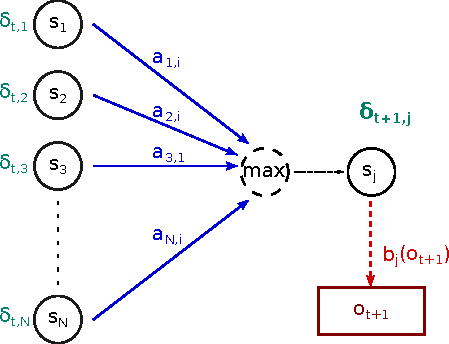
\includegraphics[width=\textwidth]{graphics/viterbi/general/viterbi-path.pdf}
    }
  \end{columns}
\end{frame}

\begin{frame}
  \frametitle{Algoritmul Viterbi - Privire de ansamblu}
  \begin{block}{Pași înainte}
    Calculăm cea mai mare probabilitate de a ajunge în starea $s_i$ 
    la momentul $t$ pe baza celor mai mari probabilități de a fi ajuns în 
    toate stările $s_j$ la $t-1$.
  \end{block}
  \pause
  \begin{block}{La final ($t=T$)}
    Starea finală este acea stare $s_i$ cu cea mai mare probabilitate de a ajunge
    la ea după observarea tuturor valorilor.
  \end{block}
  \pause
  \begin{block}{Pași înapoi}
    Refacem \emph{cea mai bună cale} alegând pentru fiecare moment $t$ starea care a
    dus la probabilitatea maximă pentru starea de la $t+1$.
  \end{block}
\end{frame}

\begin{frame}
  \frametitle{Algoritmul Viterbi (I)}
  \begin{description}
  \item[1] Inițializare: \\
    \begin{equation}
      \label{eq:viterbi-initialization}
      \begin{split}
        \delta_{1,i} & = \pi_{i}b_i(o_1), \quad 1 \le i \le N \\
        \psi_{1,i} & = 0
      \end{split}
    \end{equation}
  \item[2] Recursivitate: \\
    \begin{equation}
      \label{eq:viterbi-recursion}
      \begin{split}
        \delta_{t,j} & = [\underset{i }{\operatorname{max}}\; \delta_{t-1,i} \cdot
        a_{i,j}] \cdot b_{j}(o_{t})
        \quad \scriptstyle{2 \le t \le T, 1 \le j \le N} \\
        \psi_{t,i} & = \underset{i}{\operatorname{argmax}}\; \delta_{t-1,i}\cdot
        a_{i,j} \quad \scriptstyle{2 \le t \le T, 1 \le j \le N}
      \end{split}
    \end{equation}
  \end{description}
\end{frame}

\begin{frame}
  \frametitle{Algoritmul Viterbi (II)}
  \begin{description}
  \item[3] Terminare: \\
    \begin{equation}
      \label{eq:viterbi-termination}
      \begin{split}
        P(Q_{\text{best}} \vert O, \lambda) & = \underset{i}{\operatorname{max}}\; \delta_{T,i} \\
        q_{T_{\text{best}}} & = \underset{i}{\operatorname{argmax}}\; \delta_{T,i}
      \end{split}
    \end{equation}
  \item[4] Backtracking: \\
    \begin{equation}
      \label{eq:viterbi-backtracking}
      q_{t_{\text{best}}} = \psi_{t+1}(q_{t+1_{\text{best}}}), \quad \scriptstyle{t=T-1,T-2,\cdots, 1}
    \end{equation}
  \end{description}
\end{frame}

\begin{frame}
  \frametitle{Probleme numerice}
  \begin{itemize}
  \item Cine este $P(Q_{\text{best}} \vert O, \lambda)$?
    \begin{equation*}
      \begin{split}
        P(Q_{\text{best}} \vert O, \lambda) & = \delta_{T,i_T} \\
        P(Q_{\text{best}} \vert O, \lambda) & = \delta_{T-1,i_{T-1}} \cdot a_{i_{T-1},i_T} 
        \cdot b_{T}(o_{T})\\
        P(Q_{\text{best}} \vert O, \lambda) & = \delta_{T-2,i_{T-2}} \cdot a_{i_{T-2},i_{T-1}}
        \cdot b_{T-1}(o_{T-1}) \cdot a_{i_{T-1},j_T} \cdot b_{T}(o_{T})\\
        P(Q_{\text{best}} \vert O, \lambda) & = \displaystyle\prod \ldots
      \end{split}
    \end{equation*}
  \item Cum putem evita apropierea rapidă de zero?\pause
  \item Calculăm \alert{$log(P)$}
    \begin{equation*}
      \begin{split}
        \log(P(Q_{\text{best}} \vert O, \lambda)) & = \log(\delta_{T,i_T}) \\
        \log(P(Q_{\text{best}} \vert O, \lambda)) & = \log(\delta_{T-1,i_{T-1}}) + \log(a_{i_{T-1},i_T})
        + \log(b_{T}(o_{T}))\\
        \log(P(Q_{\text{best}} \vert O, \lambda)) & = \log(\delta_{T-2,i_{T-2}}) + \log(a_{i_{T-2},i_{T-1}})
        +\log(b_{T-1}(o_{T-1})+\log(a_{i_{T-1},j_T})+\log(b_{T}(o_{T}))\\
        \log(P(Q_{\text{best}} \vert O, \lambda)) & = \displaystyle\sum \ldots
      \end{split}
    \end{equation*}
    
  \end{itemize}
\end{frame}

\begin{frame}
  \frametitle{Probleme numerice - Rezolvare}
  \begin{itemize}
  \item Notație:
    \begin{equation*}
      \phi_{t,i}=\underset{q_1,\ldots,q_{t-1}}{\operatorname{max}}
      \log(P(q_1,\ldots,q_{t-1},q_t=s_i,o_1,\ldots,o_t\vert \lambda))=\log(\delta_{t,i})
    \end{equation*}
  \item Matricele $\log(\Pi)$, $\log(A)$ și $\log(B)$ pot fi precalculate.
  \end{itemize}
\end{frame}

\begin{frame}
  \frametitle{Algoritmul Viterbi - $log(P)$ (I)}
  \begin{description}
  \item[1] Inițializare: \\
    \begin{equation}
      \label{eq:viterbi-initialization}
      \begin{split}
        \phi_{1,i} & = \log(\pi_{i}) \mathbf{+} \log(b_i(o_1)), \quad 1 \le i \le N \\
        \psi_{1,i} & = 0
      \end{split}
    \end{equation}
  \item[2] Recursivitate: \\
    \begin{equation}
      \label{eq:viterbi-recursion}
      \begin{split}
        \phi_{t,j} & = [\underset{i}{\operatorname{max}}\; \phi_{t-1,i} \mathbf{+}
        log(a_{i,j})] \mathbf{+} \log(b_{j}(o_{t}))
        \quad \scriptstyle{2 \le t \le T, 1 \le j \le N} \\
        \psi_{t,i} & = \underset{i}{\operatorname{argmax}}\; \phi_{t-1,i} \mathbf{+}
        \log(a_{i,j}) \quad \scriptstyle{2 \le t \le T, 1 \le j \le N}
      \end{split}
    \end{equation}
  \end{description}
\end{frame}

\begin{frame}
  \frametitle{Algoritmul Viterbi - $log(P)$ (II)}
  \begin{description}
  \item[3] Terminare: \\
    \begin{equation}
      \label{eq:viterbi-termination}
      \begin{split}
        \log(P(Q_{\text{best}} \vert O, \lambda)) & = \underset{i}{\operatorname{max}}\; \phi_{T,i} \\
        q_{T_{\text{best}}} & = \underset{i}{\operatorname{argmax}}\; \phi_{T,i}
      \end{split}
    \end{equation}
  \item[4] Backtracking: \\
    \begin{equation}
      \label{eq:viterbi-backtracking}
      q_{t_{\text{best}}} = \psi_{t+1}(q_{t+1_{\text{best}}}), \quad \scriptstyle{t=T-1,T-2,\cdots, 1}
    \end{equation}
  \end{description}
\end{frame}

\begin{frame}
  \frametitle{Înapoi la exemplu}
  \begin{itemize}
  \item Să reluăm exemplul cu robotul.
  \item Robotul a recunoscut secvența de gesturi:\\
      \alert{(zâmbet $\vert$ rânjet)} $\longrightarrow$ \alert{(zâmbet $\vert$ rânjet)} $\longrightarrow$ \alert{încruntare}
  \item Am stabilit:
    $P(O \vert \lambda^{1}) > P(O \vert \lambda^{2})$\pause\\
    Deci, robotul se confruntă \emph{[, probabil]} cu un morocănos!\\
  \item A doua întrebare: \textbf{Prin ce stări a trecut acesta?}
  \end{itemize}
\end{frame}

\begin{frame}%
  \frametitle{Jovialul}%
  \begin{columns}[T]%
    \column{0.70\textwidth}%
    \only<1>{\framebox{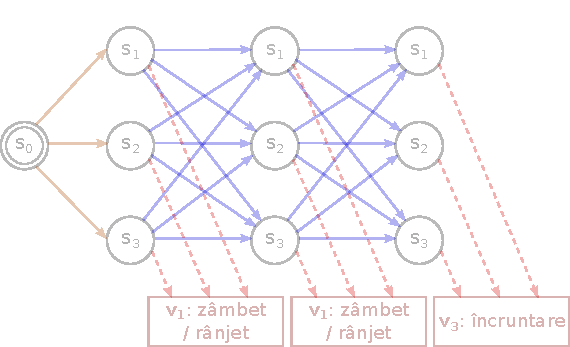
\includegraphics[width=\textwidth]{graphics/viterbi/compute-viterbi/compute-viterbi-none.pdf}}}%
    \only<2>{\framebox{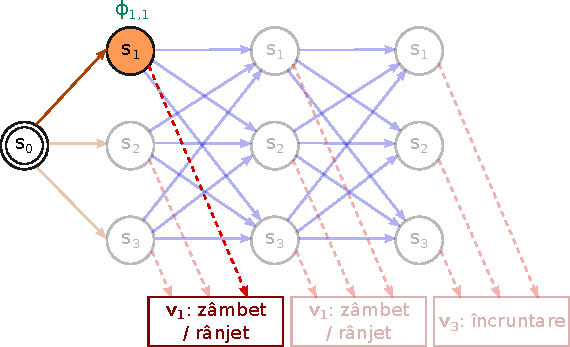
\includegraphics[width=\textwidth]{graphics/viterbi/compute-viterbi/compute-viterbi-11.pdf}}}%
    \only<3>{\framebox{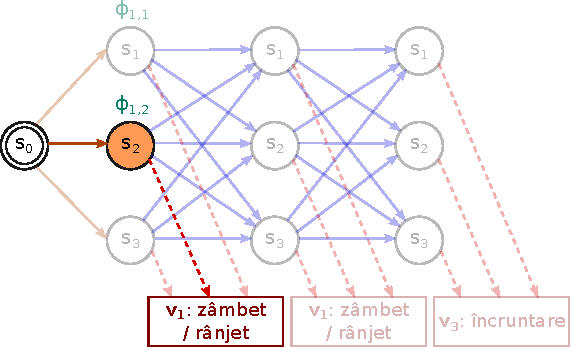
\includegraphics[width=\textwidth]{graphics/viterbi/compute-viterbi/compute-viterbi-12.pdf}}}%
    \only<4>{\framebox{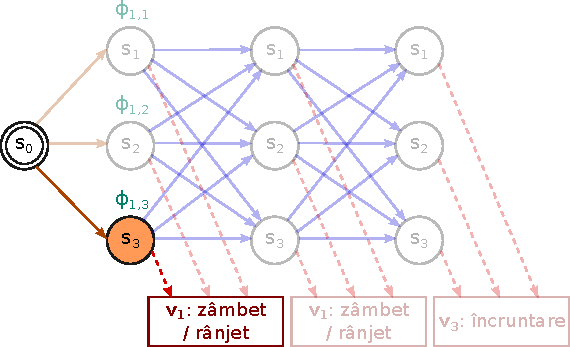
\includegraphics[width=\textwidth]{graphics/viterbi/compute-viterbi/compute-viterbi-13.pdf}}}%
    \only<5>{\framebox{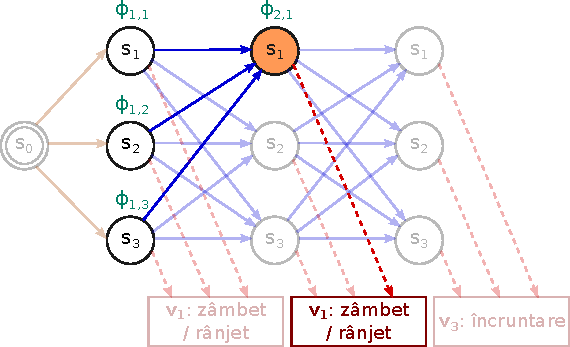
\includegraphics[width=\textwidth]{graphics/viterbi/compute-viterbi/compute-viterbi-21a.pdf}}}%
    \only<6>{\framebox{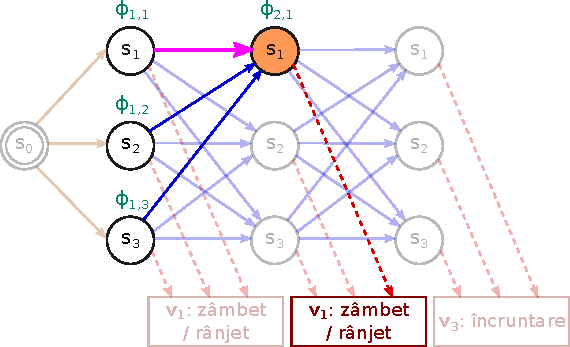
\includegraphics[width=\textwidth]{graphics/viterbi/compute-viterbi/compute-viterbi-21b.pdf}}}%
    \only<7>{\framebox{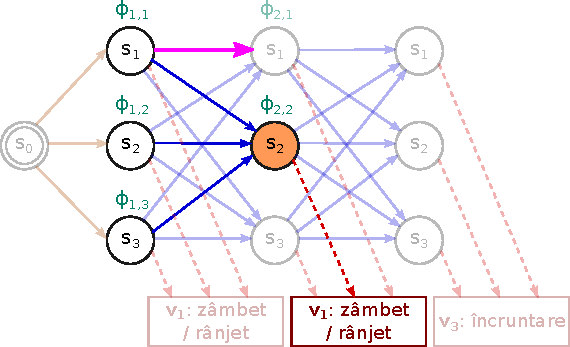
\includegraphics[width=\textwidth]{graphics/viterbi/compute-viterbi/compute-viterbi-22a.pdf}}}%
    \only<8>{\framebox{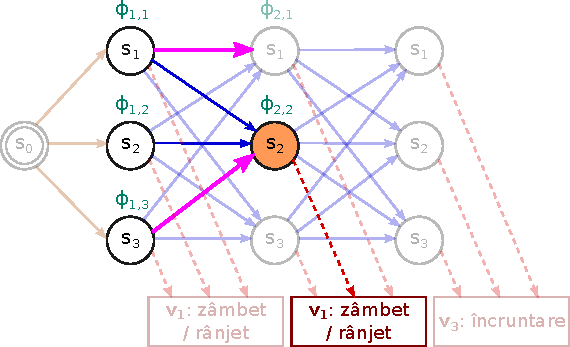
\includegraphics[width=\textwidth]{graphics/viterbi/compute-viterbi/compute-viterbi-22b.pdf}}}%
    \only<9>{\framebox{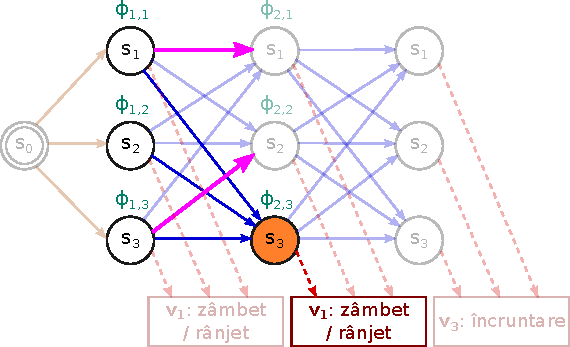
\includegraphics[width=\textwidth]{graphics/viterbi/compute-viterbi/compute-viterbi-23a.pdf}}}%
    \only<10>{\framebox{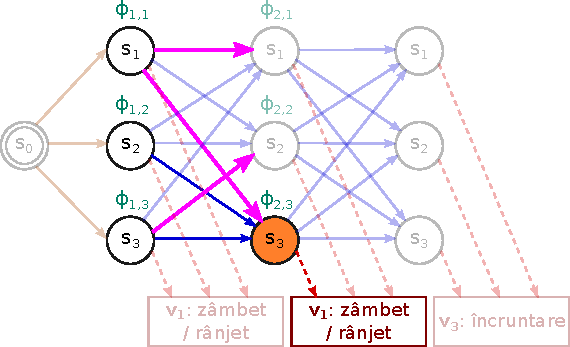
\includegraphics[width=\textwidth]{graphics/viterbi/compute-viterbi/compute-viterbi-23b.pdf}}}%
    \only<11>{\framebox{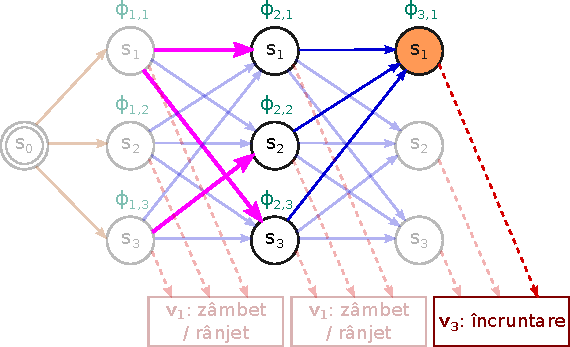
\includegraphics[width=\textwidth]{graphics/viterbi/compute-viterbi/compute-viterbi-31a.pdf}}}%
    \only<12>{\framebox{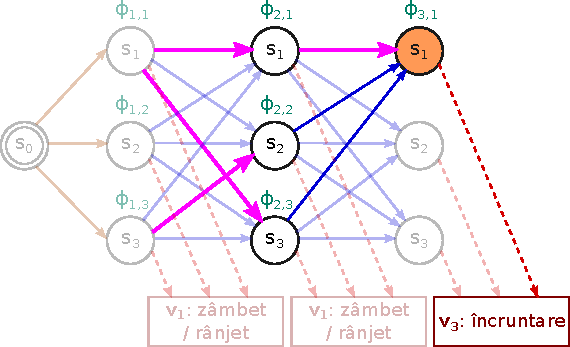
\includegraphics[width=\textwidth]{graphics/viterbi/compute-viterbi/compute-viterbi-31b.pdf}}}%
    \only<13>{\framebox{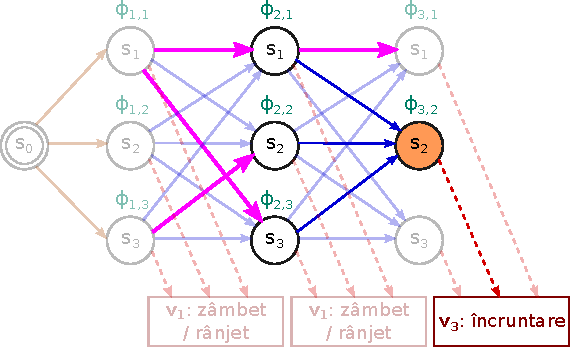
\includegraphics[width=\textwidth]{graphics/viterbi/compute-viterbi/compute-viterbi-32a.pdf}}}%
    \only<14>{\framebox{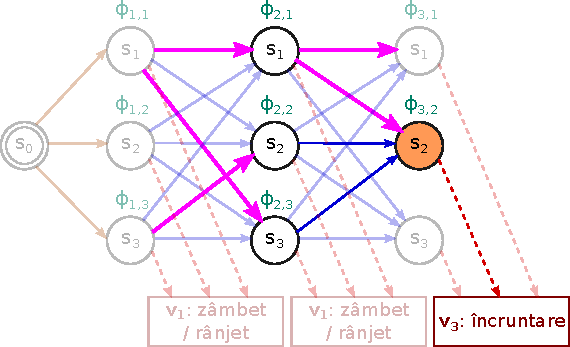
\includegraphics[width=\textwidth]{graphics/viterbi/compute-viterbi/compute-viterbi-32b.pdf}}}%
    \only<15>{\framebox{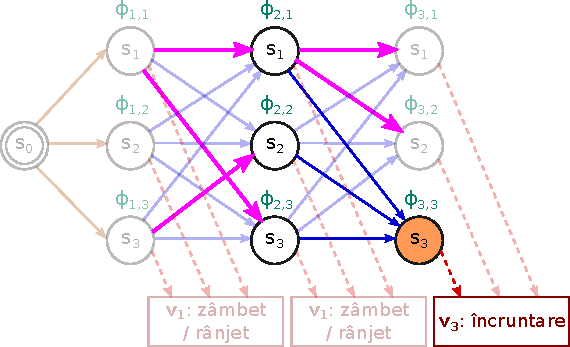
\includegraphics[width=\textwidth]{graphics/viterbi/compute-viterbi/compute-viterbi-33a.pdf}}}%
    \only<16>{\framebox{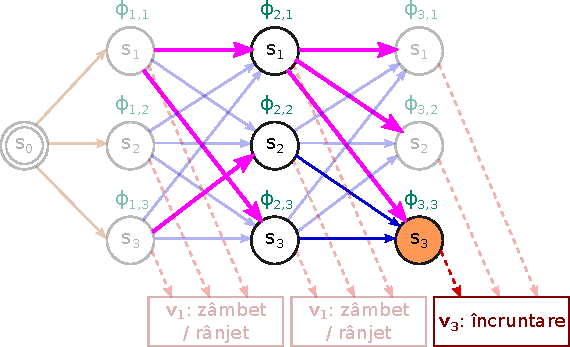
\includegraphics[width=\textwidth]{graphics/viterbi/compute-viterbi/compute-viterbi-33b.pdf}}}%
    \only<17>{\framebox{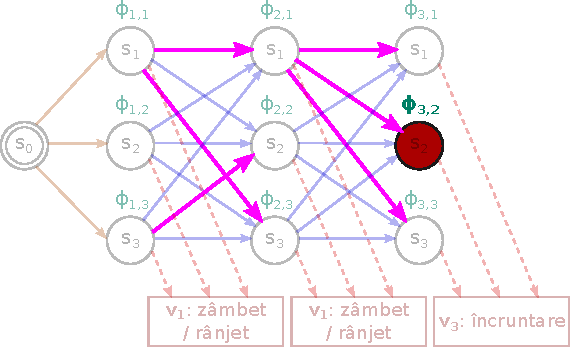
\includegraphics[width=\textwidth]{graphics/viterbi/compute-viterbi/compute-viterbi-3.pdf}}}%
    \only<18>{\framebox{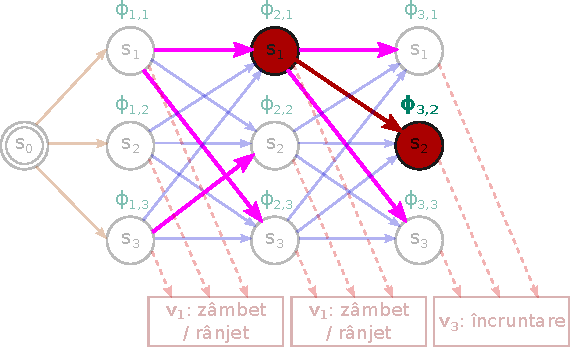
\includegraphics[width=\textwidth]{graphics/viterbi/compute-viterbi/compute-viterbi-2.pdf}}}%
    \only<19>{\framebox{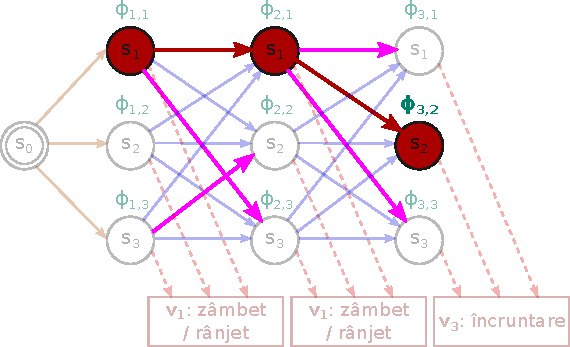
\includegraphics[width=\textwidth]{graphics/viterbi/compute-viterbi/compute-viterbi-1.pdf}}}%
    \column{0.30\textwidth}%
    \only<2>{%
      \begin{equation*}
        \begin{split}
          \scriptstyle \phi_{1,1} & \scriptstyle  = \log(\pi_{1}) + \log(b_{1,1})
      \end{split}
    \end{equation*}
    \vspace*{2em}
    \begin{equation*}
      \begin{split}
        \scriptstyle \psi_{1,1} & \scriptstyle  = 0
      \end{split}
    \end{equation*}
    }\only<3>{%
      \begin{equation*}
      \begin{split}
        \scriptstyle \phi_{1,2} & \scriptstyle  = \log(\pi_{2}) + \log(b_{2,1})
      \end{split}
    \end{equation*}
    \vspace*{2em}
    \begin{equation*}
      \begin{split}
        \scriptstyle \psi_{1,2} & \scriptstyle  = 0
      \end{split}
    \end{equation*}
    }\only<4>{%
      \begin{equation*}
      \begin{split}
        \scriptstyle \phi_{1,3} & \scriptstyle  = \log(\pi_{3}) + \log(b_{3,1})
      \end{split}
    \end{equation*}
    \vspace*{2em}
    \begin{equation*}
      \begin{split}
        \scriptstyle \psi_{1,3} & \scriptstyle  = 0
      \end{split}
    \end{equation*}
    }\only<5>{%
      \begin{equation*}
      \begin{split}
        \scriptstyle \phi_{1,3} & \scriptstyle  = \operatorname{max} \Big\lbrace \\
        \scriptstyle & \scriptstyle \log(\phi_{1,1}) + \log(a_{1,1}),\\ 
        \scriptstyle & \scriptstyle \log(\phi_{2,1}) + \log(a_{2,1}),\\
        \scriptstyle & \scriptstyle \log(\phi_{1,3}) + \log(a_{3,1}) \Big\rbrace \\ 
        \scriptstyle & \scriptstyle + \log(b_{1,1})
      \end{split}
    \end{equation*}
    % \begin{equation*}
    %   \begin{split}
    %     \scriptstyle \psi_{1,3} & \scriptstyle  = \operatorname{argmax} \Big\lbrace \\
    %     \scriptstyle & \scriptstyle \log(\phi_{1,1}) + \log(a_{1,1}),\\ 
    %     \scriptstyle & \scriptstyle \log(\phi_{2,1}) + \log(a_{2,1}),\\
    %     \scriptstyle & \scriptstyle \log(\phi_{1,3}) + \log(a_{3,1}) \Big\rbrace \\
    %   \end{split}
    % \end{equation*}
    }


  \end{columns}
  $\Phi=\begin{bmatrix}
       \scriptstyle \visible<2->{-2.1202} & \scriptstyle \visible<3->{-Inf} & \scriptstyle \visible<4->{-2.1202} \\
       \scriptstyle \visible<5->{-3.7297} & \scriptstyle \visible<7->{-Inf} & \scriptstyle \visible<9->{-4.2205} \\
       \scriptstyle \visible<11->{-6.7254} & \scriptstyle \visible<13->{-5.1567} & \scriptstyle \visible<15->{-5.3391}\end{bmatrix}$ $\Psi=\begin{bmatrix}
       \scriptstyle \visible<2->{0} & \scriptstyle \visible<3->{0} & \scriptstyle \visible<4->{0} \\
       \scriptstyle \visible<6->{1} & \scriptstyle \visible<8->{3} & \scriptstyle \visible<10->{1} \\
       \scriptstyle \visible<12->{1} & \scriptstyle \visible<14->{3} & \scriptstyle \visible<16->{1}\end{bmatrix}$ $Q_{best} = \begin{bmatrix}\visible<19->{1} & \visible<18->{1} & \visible<17->{2}\end{bmatrix}$
     
\end{frame}

\begin{frame}[fragile]
  \frametitle{Algoritmul Viterbi}
  \begin{algorithm}[H]
    \scriptsize
    \caption{Calculul celei mai probabile secvențe $Q_{\text{best}}$}
    \label{alg:viterbi}
    \algsetup{linenosize=\tiny} \algsetup{indent=2.25em}
    \begin{algorithmic}[2]
      \FOR{$i=1$ to $N$}
      \STATE $\phi_{1,i}$ $\leftarrow$ $\log(\pi_{i}) + \log(b_i(o_1))$
      \STATE $\psi_{1,i}$ $\leftarrow$ $0$
      \ENDFOR
      \FOR{$t=2$ to $T$}
      \FOR{$i=1$ to $N$}
      \STATE $\phi_{t,j}$ $\leftarrow$ $[\underset{i}{\operatorname{max}}\; \phi_{t-1,i} +
      log(a_{i,j})] + \log(b_{j}(o_{t}))$
      \STATE $\psi_{t,i}$ $\leftarrow$ $\underset{i}{\operatorname{argmax}}\; \phi_{t-1,i} +
      \log(a_{i,j})$
      \ENDFOR
      \ENDFOR
      \STATE $\log(P(Q_{\text{best}} \vert O, \lambda))$ $\leftarrow$ $\underset{i}{\operatorname{max}}\; \phi_{T,i}$
      \STATE $q_{T_{\text{best}}}$ $\leftarrow$ $\underset{i}{\operatorname{argmax}}\; \phi_{T,i}$
      \FOR{$t=T-1$ to $1$}
      \STATE $q_{t_{\text{best}}}$ $\leftarrow$ $\psi_{t+1}(q_{t+1_{\text{best}}})$
      \ENDFOR
    \end{algorithmic}
  \end{algorithm}
\end{frame}

\begin{frame}
  \frametitle{A venit vremea să scriem cod}
  \begin{enumerate}
  \item Faceți o copie a fișierului \texttt{viterbi\_disc.m.stub} 
    și denumiți-o \texttt{viterbi\_disc.m} (eliminați sufixul \texttt{.stub}).
    \\Veți implementa funcția:\\
    \mcode{function [logP, Q] = viterbi_disc(O,Pi, A, B)}
    \pause
  \item Completați cele două secțiuni.%
    \vspace*{-1em}
    \lstinputlisting{m-files/viterbi.m}
\item Folosiți \mcode{hmm_test} pentru a vă testa codul.
\end{enumerate}
\end{frame}
